\eventsection{METODOLOGIA}

\eventsubsection{\'Area de estudo e dados}

O estudo foi desenvolvido a partir de medi\c{c}\~oes realizadas no Lago do Serpa, localizado em Itacoatiara, no estado do Amazonas. O material utilizado foi organizado a partir de pontos georreferenciados de coleta, reunindo informa\c{c}\~oes f\'isico-qu\'imicas da \'agua e atributos associados ao ambiente amostrado, disponibilizados no conjunto de dados georreferenciado publicado em Mendeley Data \cite{assuncao2026dataset}. Neste artigo, o foco recai sobre tr\^es indicadores de interesse para o acompanhamento ambiental: pH, oxig\^enio dissolvido e turbidez.

\begin{figure}[htbp]
\centering
\caption{Caracteriza\c{c}\~ao visual e territorial da \'area de estudo no Lago do Serpa.}
\label{fig:area_estudo}
\begin{subfigure}[t]{0.46\textwidth}
\centering
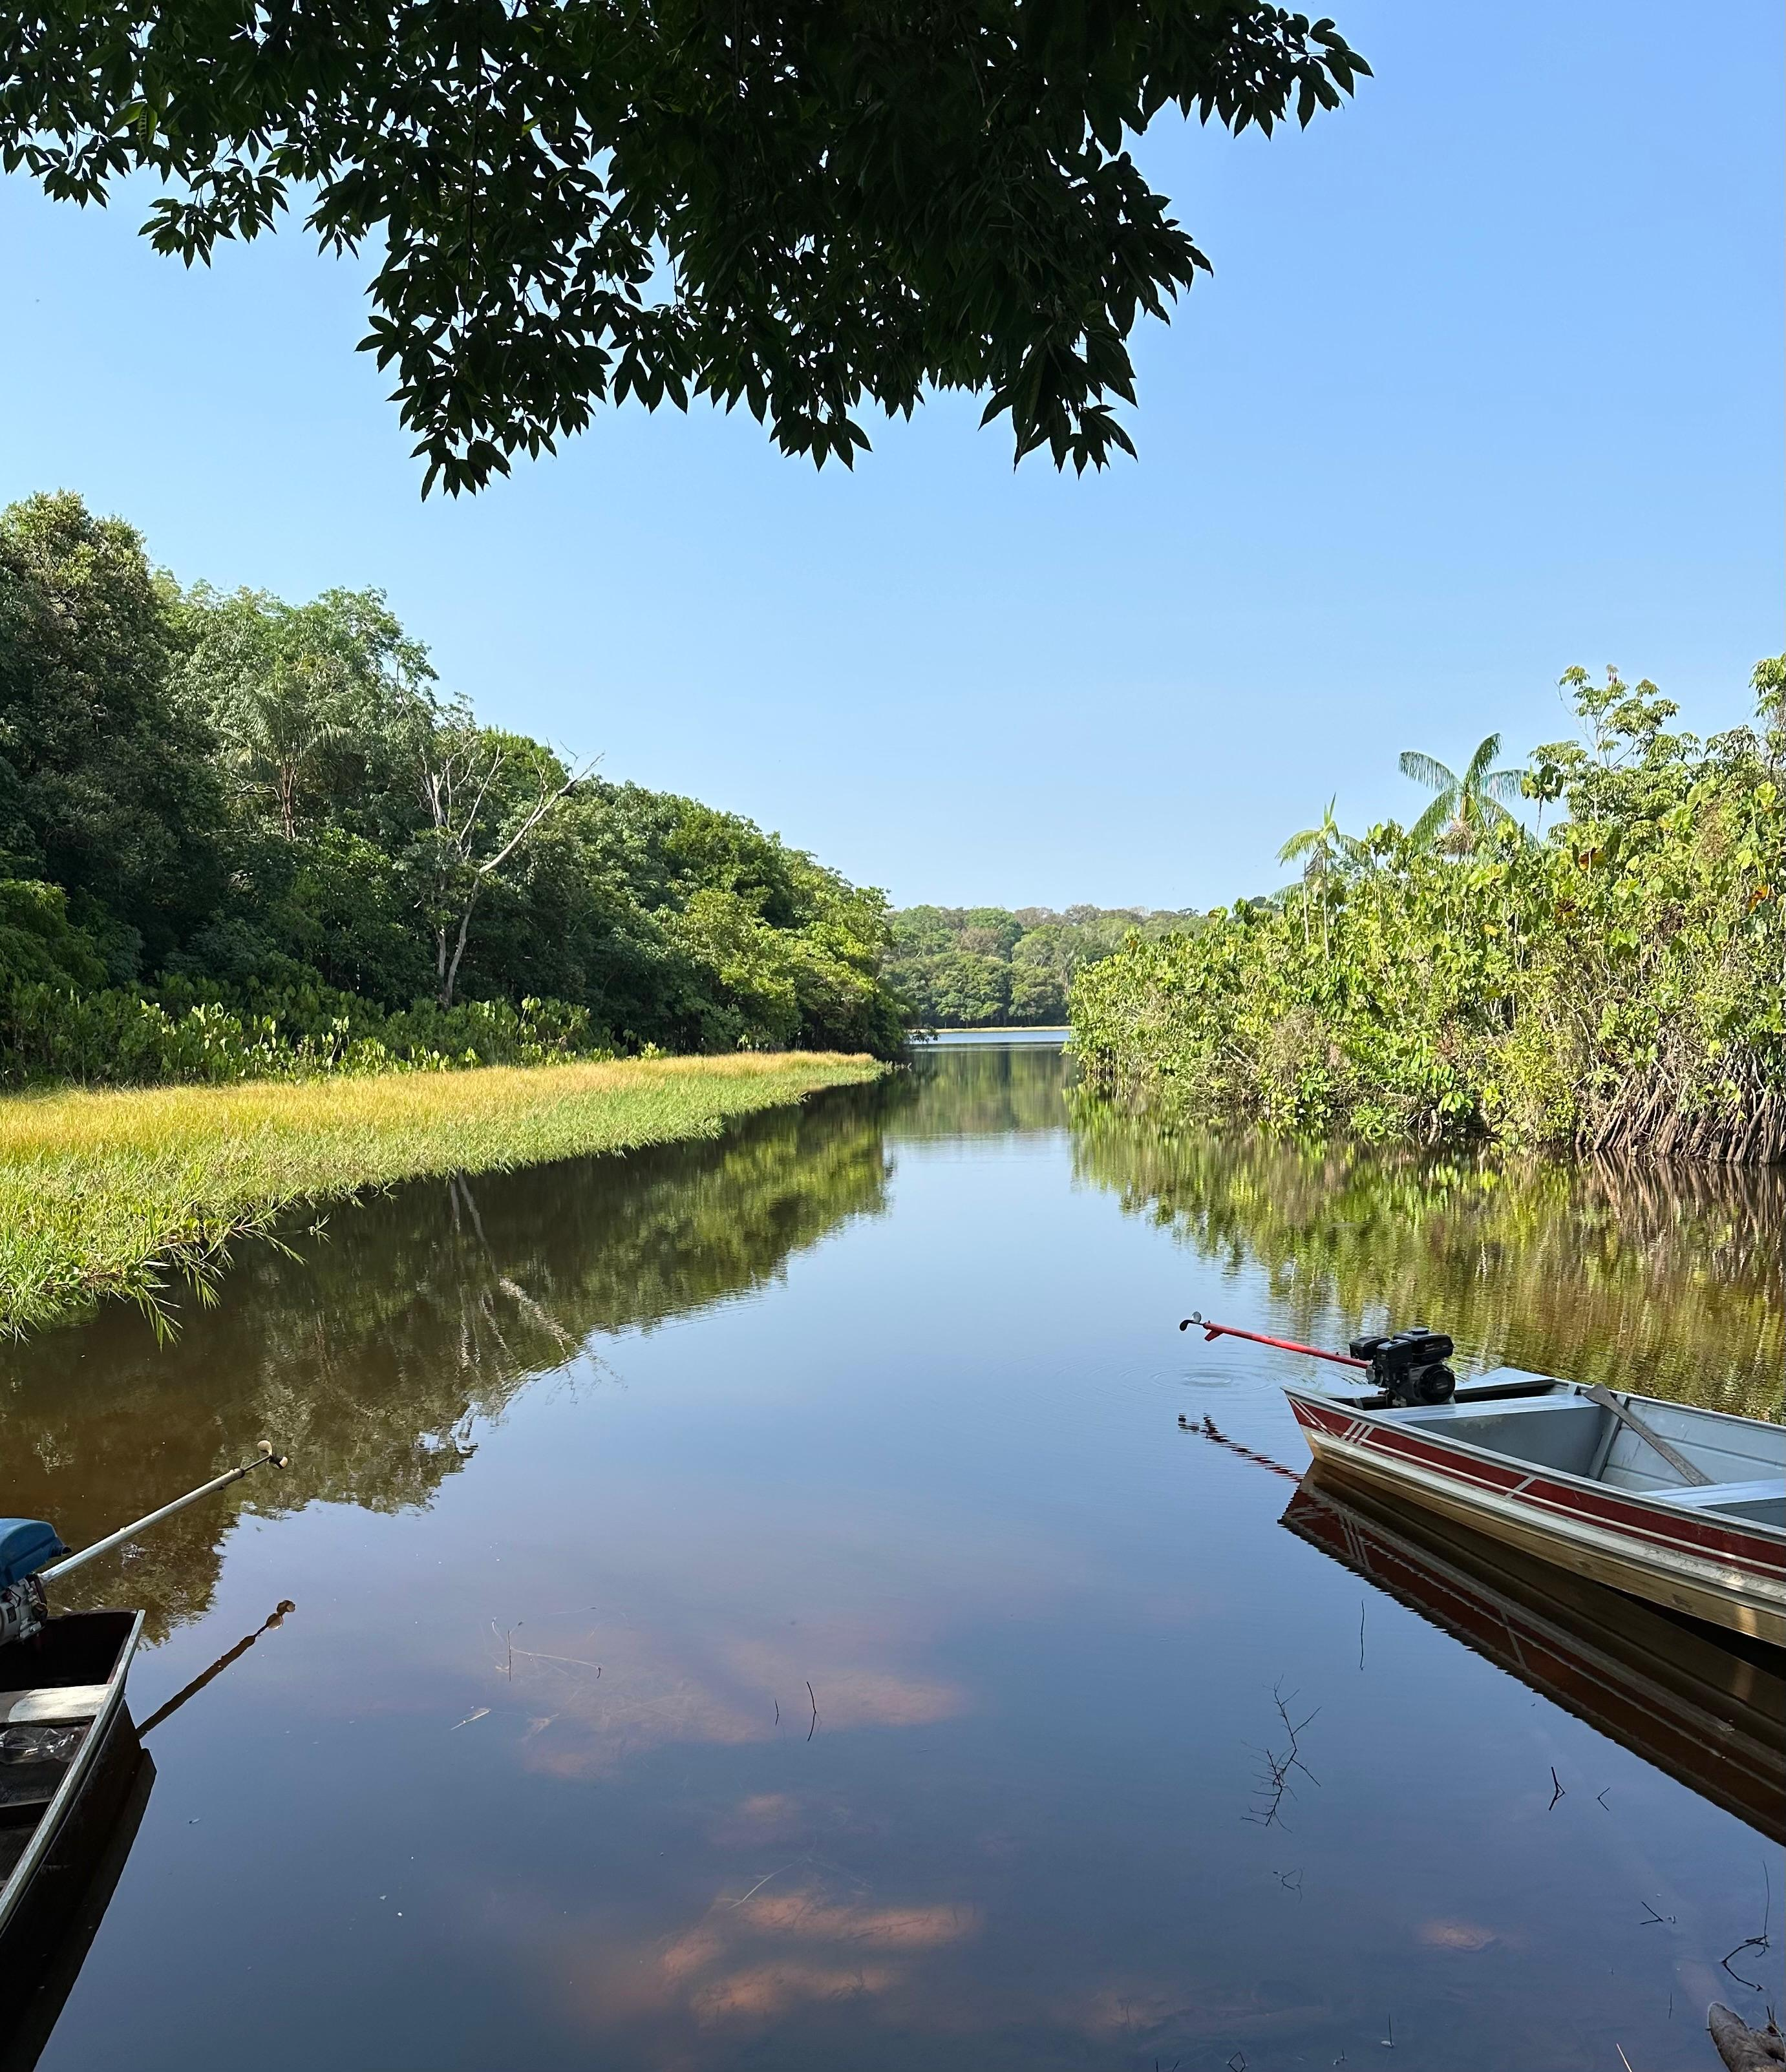
\includegraphics[width=\textwidth]{foto_lago_serpa_clean.jpg}
\caption{Registro visual da \'area estudada}
\end{subfigure}
\hfill
\begin{subfigure}[t]{0.52\textwidth}
\centering
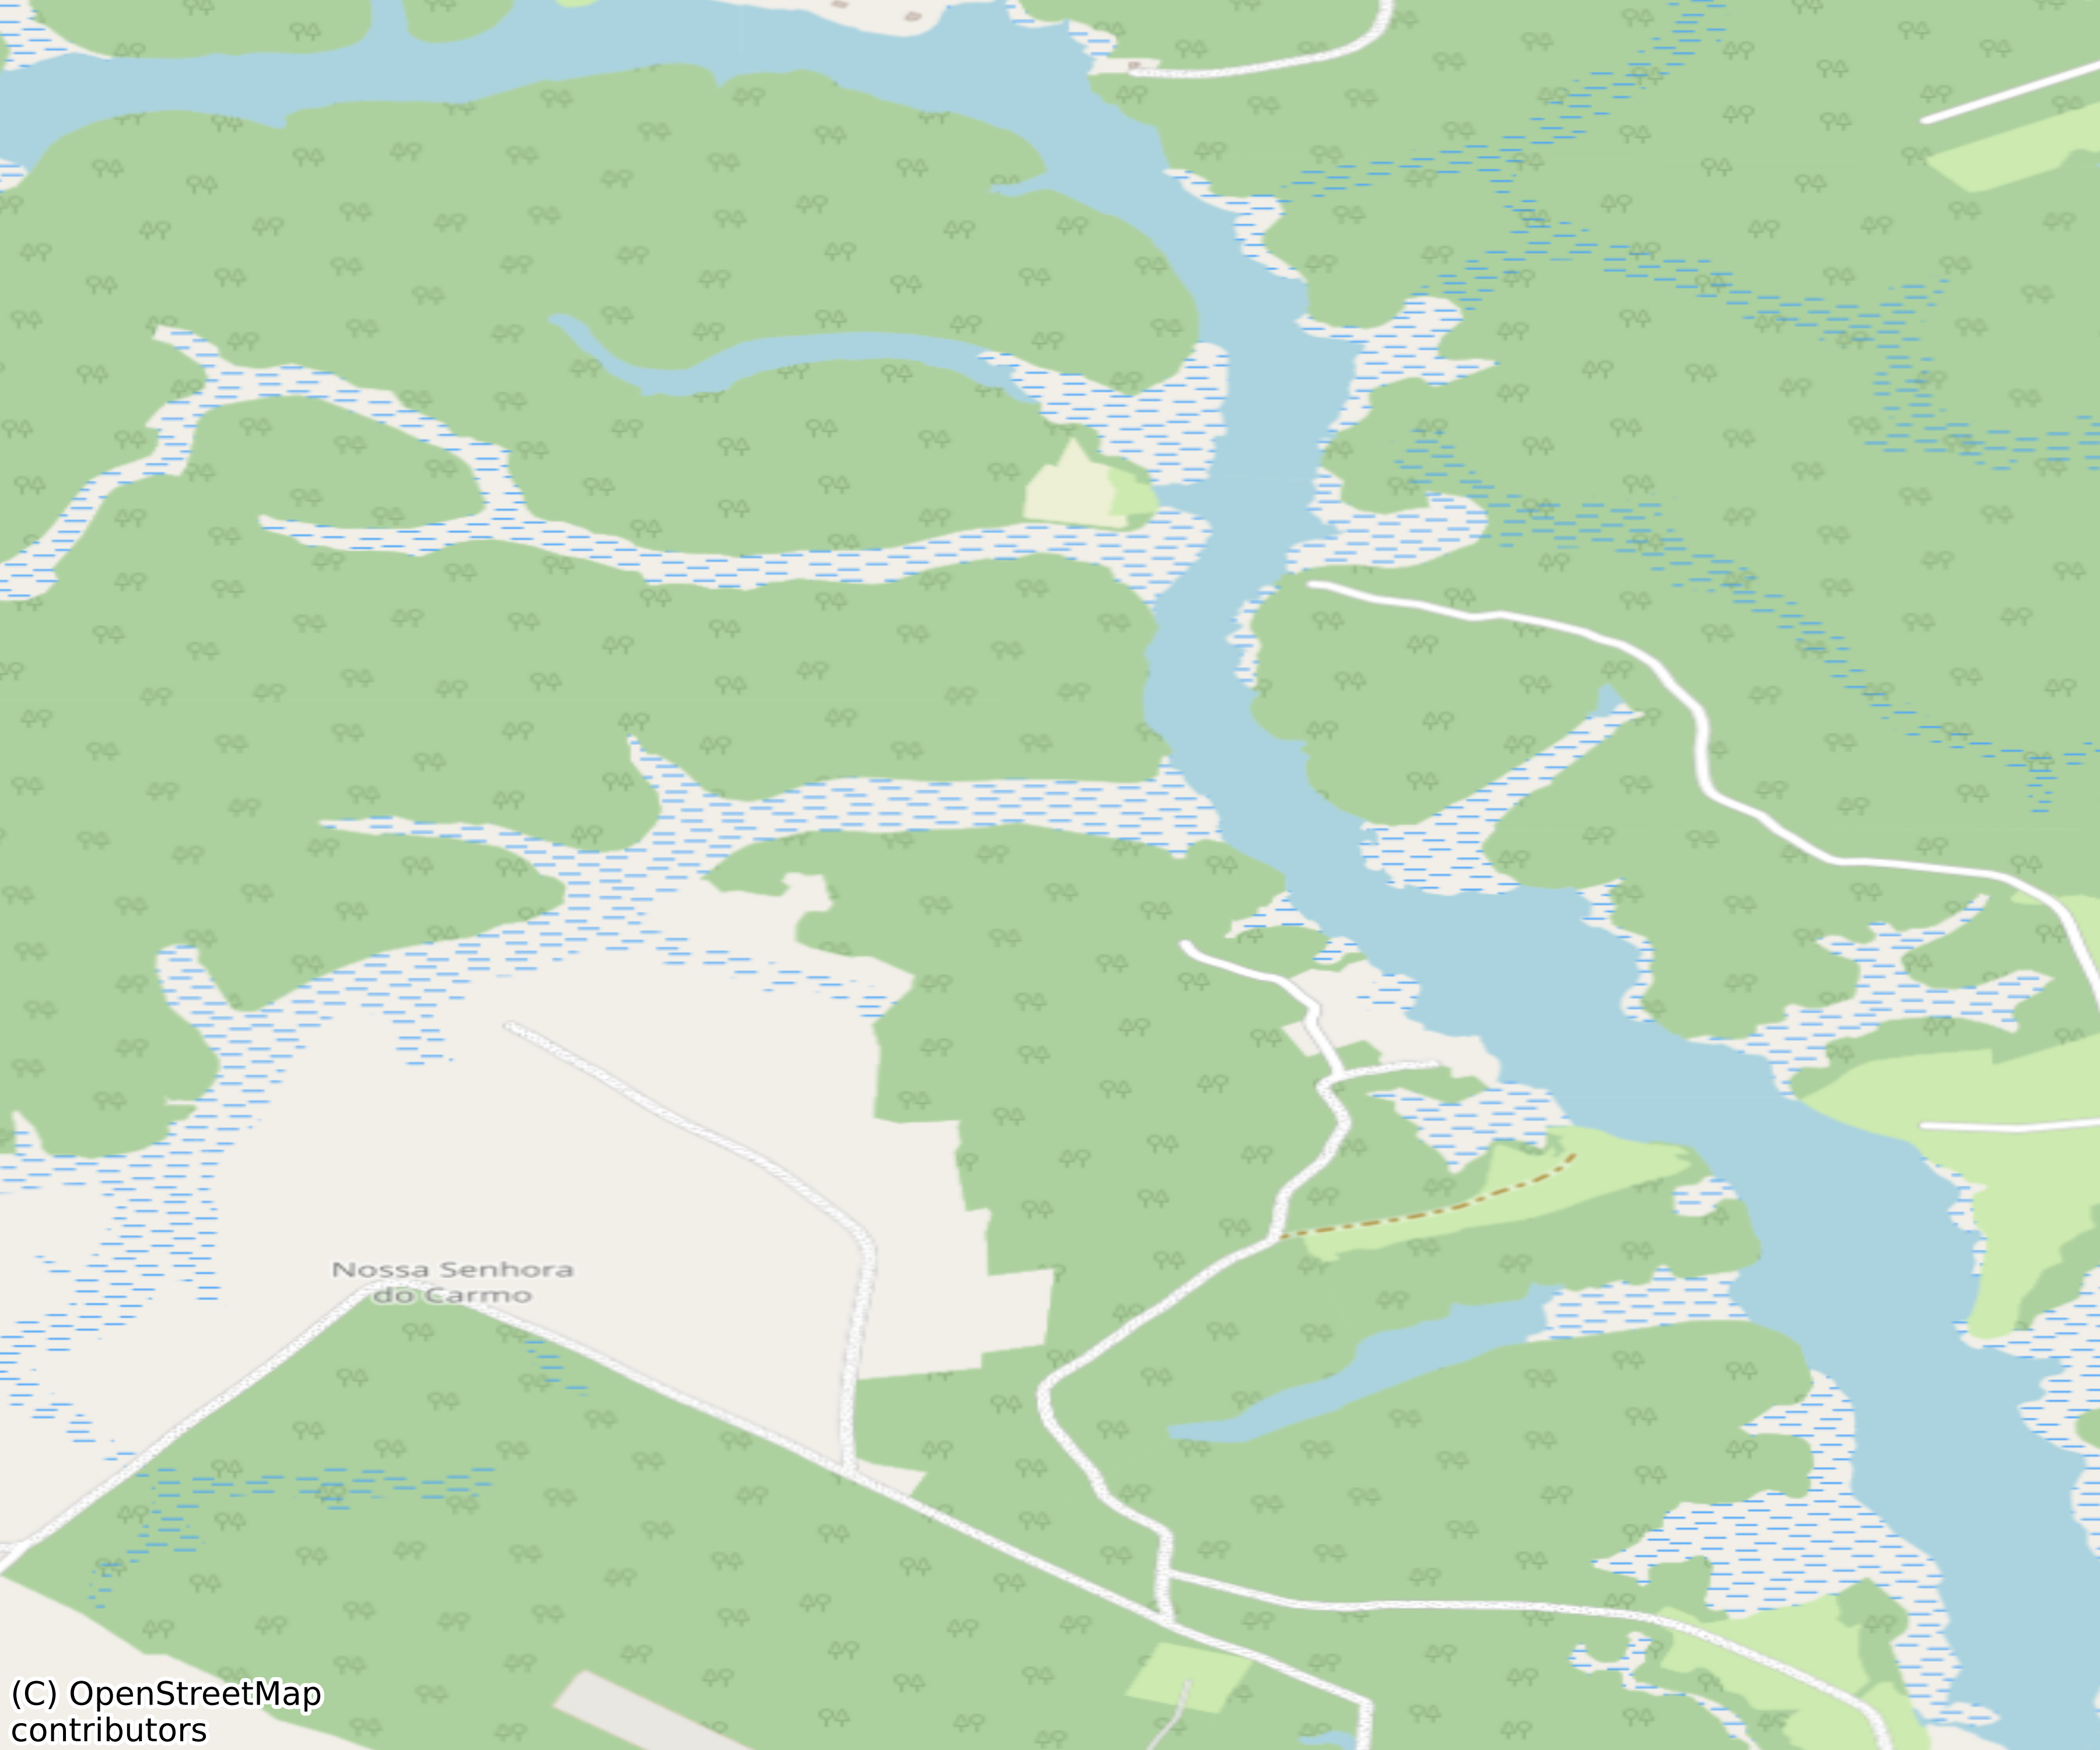
\includegraphics[width=\textwidth]{map_basemap_osm_21S_clean_copy.png}
\caption{Contexto territorial em base cartogr\'afica}
\end{subfigure}
\artigofonte{acervo do estudo de campo e elabora\c{c}\~ao pr\'opria com base em OpenStreetMap.}
\end{figure}

Os dados passaram por etapas de organiza\c{c}\~ao, confer\^encia e padroniza\c{c}\~ao para permitir uso consistente no sistema. Em seguida, o conjunto foi distribu\'ido em etapas de desenvolvimento e verifica\c{c}\~ao da solu\c{c}\~ao, conforme o protocolo adotado no estudo de base. Embora se trate de uma base local, seu valor est\'a no fato de representar um ambiente amaz\^onico real e de permitir a verifica\c{c}\~ao da proposta em condi\c{c}\~oes pr\'oximas do uso em campo.

\eventsubsection{Sistema embarcado proposto}

O sistema proposto foi concebido para funcionar sem depend\^encia de conex\~ao permanente com a internet. Sua l\'ogica de opera\c{c}\~ao pode ser resumida em tr\^es etapas: recebimento dos dados de entrada, processamento local por um modelo de intelig\^encia artificial e apresenta\c{c}\~ao dos resultados ao usu\'ario. Essa organiza\c{c}\~ao permite que o processamento ocorra no pr\'oprio dispositivo, o que \'e especialmente relevante para comunidades ribeirinhas e regi\~oes remotas com baixa conectividade.

Para verificar a viabilidade da proposta, o sistema foi preparado para execu\c{c}\~ao em diferentes plataformas de borda. Foram considerados dispositivos com perfis distintos de uso: smartphones Android, voltados \`a intera\c{c}\~ao em campo; Raspberry Pi, adequada a esta\c{c}\~oes locais de monitoramento; e ESP32, representando um cen\'ario de hardware compacto e de baixo custo.

Essa variedade de plataformas permite observar a solu\c{c}\~ao em condi\c{c}\~oes pr\'aticas distintas. Em um cen\'ario, a prioridade pode ser a visualiza\c{c}\~ao local e a facilidade de uso; em outro, pode ser a implanta\c{c}\~ao em dispositivos pequenos e simples. Assim, a metodologia foi estruturada para avaliar a capacidade de adapta\c{c}\~ao do sistema a diferentes rotinas de monitoramento ambiental, sem concentrar a discuss\~ao em detalhes internos do modelo.

\eventsubsection{Procedimentos de avalia\c{c}\~ao}

A avalia\c{c}\~ao foi conduzida em duas frentes complementares. A primeira considerou a capacidade do sistema de estimar os par\^ametros de interesse a partir dos dados dispon\'iveis. A segunda observou sua execu\c{c}\~ao em plataformas embarcadas, levando em conta medidas de lat\^encia e vaz\~ao de infer\^encia. O objetivo n\~ao foi apenas verificar se o sistema produz bons resultados num\'ericos, mas se esses resultados podem ser efetivamente aproveitados em uma rotina de monitoramento ambiental. Dessa forma, a metodologia privilegia uma leitura aplicada: al\'em de prever vari\'aveis, o sistema precisa ser vi\'avel em dispositivos reais e \'util para apoiar acompanhamento cont\'inuo, triagem ambiental, apoio \`a sa\'ude p\'ublica e identifica\c{c}\~ao de \'areas de maior aten\c{c}\~ao em regi\~oes de dif\'icil acesso.
